\chapter{Introduzione}
\begin{comment}

la scaletta dei capitoli è:
- introduzione
- stato dell'arte
- metodi e strumenti
- sviluppo del progetto
- risultati

Sottosezioni di introduzione:
- Motivazione

    - modelli neurali per la segmentazione dei difetti
        - applicazioni
        - il dataset e i requisiti per l'addestramento

- Approccio al problema

    - La generazione di un dataset sintetico

- introduzione alle reti neurali

    - feedforward networks
        - il neurone
        - la funzione di attivazione
        - backpropagation

    - convolutional neural networks
        - la convoluzione
        - il pooling
        - l'upsampling

\end{comment}


\section{Motivazione \ok}

\subsection{Modelli neurali per la segmentazione nel controllo qualità\ok}

Oggi le reti neurali trovano un vasto impiego in moltissimi campi, dall'industria alla medicina, fino alla vita di tutti i giorni.
Il grande vantaggio che ci portano è la capacità di apprendere da un set di dati, e di generalizzare su di uno nuovo,
permettendoci di risolvere problemi che altrimenti sarebbero matematicamente troppo complessi da risolvere con un algoritmo.
Ci sono vari esempi in cui i modelli neurali raggiungono risultati superiori a quelli ottenuti dall'uomo, in determinati task, 
o almeno se non lo superano in termini di accuratezza, lo fanno in termini di velocità, scalabilità, costi e prestazioni.

Un task in cui le reti neurali eccellono è la segmentazione di immagini, ovvero la classificazione pixel per pixel di un'immagine,
questo tipo di task è utilizzato ad esempio nel campo medico per la segmentazione di organi, tumori, o in campo industriale per la segmentazione di difetti,
per la verifica automatica della qualità di un prodotto o di un semilavorato.

Nel caso specifico, per la segmentazione dei difetti l'utilizzo di questo tipo di modelli è molto diffuso, in quanto risolve un grave problema 
che affligge i reparti controllo qualità delle aziende, ovvero il calo della concentrazione al quale un operatore è soggetto dopo un certo numero di ore di lavoro.
Infatti una persona per quanto allenata e preparata, dopo un certo numero di ore di lavoro, è soggetta a stanchezza e con essa
la sua accuratezza nel riconoscere un difetto diminuisce, mentre un modello neurale adeguatamente addestrato, in condizioni ambientali stabili,
come ad esempio una adeguata illuminazione, una videocamera ad alta risoluzione e un'adeguata distanza dal soggetto, sarà in grado di mantenere 
un'accuratezza costante, senza necessità di fermarsi per riposare. Questo si traduce in un risparmio di tempo e di denaro per l'azienda,
In quanto il controllo manuale richiede più tempo ed è più soggetto ad errori, i quali spesso si trasformano in ritardi nella consegna dei prodotti,
spese di trasporto aggiuntive per il ritorno o la sostituzione del prodotto, o addirittura la perdita di un cliente.

\begin{figure}[H]
    \centering
    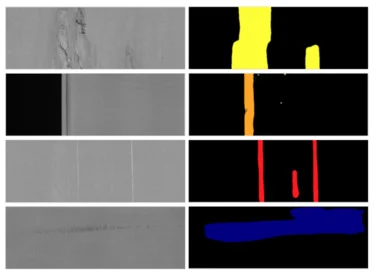
\includegraphics[width=0.4\textwidth]{imgs/segm_example_1_crop.png}
    \caption{An example of segmented defects from the "Severstal steel defect dataset".
    credits: Neven Robby and Goedemé Toon, 2021, A Multi-Branch U-Net for Steel Surface Defect Type and Severity Segmentation.
    https://www.mdpi.com/2075-4701/11/6/870}
    \label{fig:segm_example_1}
\end{figure}


\subsection{Il dataset, requisiti e problematiche di realizzazione \ok}
\begin{comment}
    Va rivisto il contenuto e integrate le parti provenienti dalla sezione precedente.
\end{comment}

La problematica di avere un modello con elevata accuratezza per task di segmentazione è relativa alla quantità e qualità dei dati necessari,
i quali raramente sono disponibili opensource o per l'acquisto, rendendo necessaria la creazione di un dataset apposito.
Molti task richiedono un grande quantità di dati per essere generalizzati correttamente, e ogni singolo esempio richiede molta concentrazione
da parte dell'annotatore in quanto non sempre i difetti sono ben visibili. 

In generale la creazione di un dataset è un'operazione molto complessa, non solo dal punto di vista dell'annotatore, ma in oltre da un punto di vista
organizzativo e logistico. Infatti ci sono diversi step che si devono seguire:
\begin{itemize}
    \item \textbf{Acquisizione delle immagini}: Le immagini devono essere acquisite in modo da avere una buona qualità, o almeno sufficiente ai fini dell'apprendimento.
        Se possibile in oltre dovrebbero avere una adeguata uniformità di condizioni (luce, distanza, ...) per garantire le migliori prestazioni da parte del modello,
        ovviamente solo se poi è possibile garantire le stesse condizioni anche nell'utilizzo finale del modello, altrimenti una grande varietà delle condizioni
        è preferibile.
    \item \textbf{Definizione delle classi}: Nel caso di dataset multi-classe, uno step molto importante è quello di scegliere accuratamente le classi
        e definire in maniera univoca l'associazione tra una classe e una particolare tipologia di difetto. Questo passaggio potrebbe sembrare banale ma in realtà
        nasconde delle grandi insidie, infatti una classificazione non adeguata andrà a causare confusione nel modello, diminuendo la sua accuratezza e/o 
        rendendo il lavoro più difficile per gli annotatori andando a rallentare il processo di annotazione o comunque a ridurne la qualità.
        Questo tipo di problematiche purtroppo si manifestano chiaramente soltanto in uno stato avanzato del progetto,
        rendendo necessarie revisioni della documentazione, modifica di tutti gli esempi già annotati, con conseguente perdita di tempo e denaro.
    \item \textbf{Definizione della documentazione}: Questo passaggio è un'estensione del precedente, e consiste nella definizione di una documentazione
        Che specifichi senza ambiguità, ad un nuovo annotatore come riconoscere senza dubbio un difetto e classificarlo nella giusta classe.
        Questa fase spesso non termina prima dell'inizio dell'annotazione, ma si protrae per tutta la durata del progetto, in quanto
        spesso nuovi casi non previsti si presentano durante l'annotazione, e la documentazione deve essere aggiornata in tempo reale.
    \item \textbf{Annotazione}: Questo è il passaggio più lungo e costoso, in quanto richiede una squadra di persone,
        che devono essere formate per lo specifico task, e che devono essere costantemente seguite per garantire la qualità del lavoro.
    \item \textbf{Revisione}: Assieme all'annotazione questo è un passaggio chiave, in quanto permette di verificare che l'annotazione sia stata fatta correttamente,
        e che non ci siano errori nell'annotazione. Spesso infatti gli annotatori acquisiscono dei bias errati nei confronti di una certa classe, o di un certo tipo di difetto, 
        che deve essere identificato e reso noto all'annotatore per correggerlo, ed evitare che questo errore si ripeta in futuro.
        Per evitare che ciò accada oltre al primo annotatore lo stesso esempio viene solitamente rivisto da 2 o 4 persone diverse.
        Si noti che gli errori degli annotatori che non vengono identificati verranno appresi dal modello finale come una corretta classificazione, ciò giustifica un tale 
        dispendio di risorse in questa fase.
\end{itemize} 

\subsection{Approccio al problema \ok}
\begin{comment}
Realizzare un architettura in grado di generare un buona quantità di dati annotati a partire da una quantità ridotta.
TODO: aggiungi paper di tecnica copy paste
\end{comment}

La creazione di un dataset come precedentemente illustrato è un processo complesso e dispendioso, che richiede molte risorse umane e finanziarie,
dunque l'intento in questo progetto è quello di proporre un approccio alternativo che sia in grado di ridurre per quanto possibile la durata e il costo
di questo lavoro.
Partendo dal presupposto che almeno in parte il dataset deve essere realizzato manualmente, la proposta è quella di realizzare una certa 
quantità di campioni manualmente seguendo lo schema già visto, per poi addestrare un modello neurale per generare ulteriori esempi sintetici,
raggiungendo un numero di esempi totali che permetta di addestrare un modello con buone prestazioni, ad un costo ridotto rispetto al caso in cui
tutti i dati fossero stati realizzati manualmente.

Per la definizione della pipeline di generazione dei dati, si è partiti dal concetto di \textit{generative adversarial network} (GAN), che è una tecnica di machine learning
che permette di generare dati sintetici utilizzando come base dati reali, tali dati sintetici possono essere utilizzati per addestrare un modello neurale.
Tale tecnica ha trovato riscontri positivi in molte ricerche pubblicate in ambito di computer vision \cite{ganbasedaugexample} , in cui i modelli GAN vengono
utilizzati per espandere il numero di immagini presenti in un dataset e migliorare la generalizzazione di un modello di classificazione.
Ovviamente gli aumenti di accuratezza, precisione e recall dipendono dal numero di esempi presenti nel dataset e dalla complessità del problema.
Tale tecnica potrebbe essere considerata una versione più sofisticata di data augmentation, in quanto permette di generare dati sintetici molto più complessi
e realistici di quelli che si possono ottenere con semplici trasformazioni geometriche o matematiche.
Per generare dati utilizzabili per addestrare un modello di segmentazione però è necessario risolvere un'ulteriore problema,
infatti un normale modello GAN, fedele alla sua definizione originale \cite{goodfellow2014generative} , è in grado di generare intere immagini,
che possono essere utilizzate per addestrare un modello di classificazione, ma non sono utilizzabili per addestrare un modello di segmentazione,
in quanto per l'addestramento di tale architettura è necessario che gli oggetti di interesse abbiano una maschera che specifichi la loro posizione.
Ci sono vari approcci di augmentation per la segmentazione che risultano molto più semplici di addestrare un modello GAN, come il caso del metodo "copy paste" \cite{ghiasi2021simple},
il quale propone come augmentation per i dataset di segmentazione la copia di un oggetto presente in un'immagine, ritagliandolo attraverso la sua maschera,
e incollandolo su di un nuovo background potenzialmente in una nuova posizione, tale metodo risulta estremamente efficacie per oggetti indipendenti dal contesto con contorni ben definiti,
ma risulta inutile nel momento in cui l'oggetto che vogliamo generare ha una interdipendenza forte con l'area immediatamente circostante,
pensiamo ad esempio un difetto su di un'auto, un graffio o una bozza, non potrà essere copiato da un'auto e incollato su di un'altra in quanto subentreranno una serie di
di artifacts, come la variazione netta di colore tra l'auto e il difetto, rischiando di introdurre un bias nel modello, il quale finirebbe per cercare la variazione netta di colore
e non più le features del difetto. Per risolvere questo problema con questa particolare categoria di dataset ci sono 2 principali strade illustrate di seguito.

\subsubsection{Generatore con architettura a solo decoder}

    Questo approccio prevede un'architettura a solo decoder, ovvero un modello che prende in ingresso un tenore di determinate dimensioni e
    che attraverso una serie di operazioni di upsampling o dilated convolution ad esempio, effettua un'espansione di tale tensore
    portandolo alle dimensioni finali. 
    Generalmente si mette in ingresso un vettore casuale di dimensione definita, ottenendo in uscita un tensore delle dimensioni di un'immagine con i canali rgb 
    ed eventualmente altri n canali per la maschere che identificano le classi desiderate.
    Un'esempio di tale architettura è illustrata di seguito.

    \begin{figure}[H]
        \centering
        \includesvg[width=0.6\textwidth]{imgs/Decoder_only.svg}
        \caption{Esempio di architettura a solo decoder.}
        \label{fig:decoder_only_architecture}
    \end{figure}

    Questo approccio risulta più semplice da implementare, lasciando però al modello il compito di imparare a generare correttamente
    le immagini e delle maschere coerenti, compito non facile, che a seconda del task può necessitare di un elevato numero di esempi. 
    Questa architettura dovrà imparare oltre alla struttura degli oggetti target, a posizionarli nell'immagine e a generare lo sfondo.
    Un'altra problematica di questo approccio è il controllo, infatti l'unico modo di interagire con tale modello è modificando il valore
    del vettore z dato in input, il quale permette di spostarsi nello spazio latente, al quale il modello associa diverse caratteristiche dell'immagine
    di output in maniera altamente non lineare, rendendo un eventuale controllo dell'output del modello molto difficile.
    La difficoltà di controllare il modello rende dunque difficoltoso o impossibile controllare, qualora fosse necessario, la posizione, l'intensità,
    la dimensione o la forma degli oggetti generati.

\subsubsection{Generatore con architettura a encoder-decoder}

    Quest'ultimo è l'approccio scelto in questo progetto, in quanto permette di avere un maggiore controllo sull'output del modello,
    anche se prevede una training pipeline più complessa da gestire.
    Al contrario del caso precedente Il modello con struttura encoder-decoder permette di passare in ingresso un'immagine base e una o più maschere
    che identificano le aree dove determinati oggetti devono essere generati, trasformando il task di generazione puro in un task di inpainting.
    I vantaggi principali di questa tecnica stanno nel fatto che il modello non deve più apprendere la distribuzione degli oggetti nello spazio dell'immagine,
    nè deve apprendere in maniera troppo approfondita i background, ma si può focalizzare maggiormente sulla struttura degli oggetti da generare.
    
    \begin{figure}[H]
        \centering
        \includesvg[width=0.8\textwidth]{imgs/Encoder_decoder.svg}
        \caption{Esempio di architettura con encoder e decoder.}
        \label{fig:encoder_decoder_architecture}
    \end{figure}

\section{Introduzione alle reti neurali \ok}
\begin{comment}
    Breve sezione che ripercorre le strutture base utilizzate in questa tipologia di reti neurali.

    indice di questa sezione:
    - Dal machine learning al deep learning

    - feedforward networks
        - il neurone
        - la funzione di trasferimento
        - Una semplice rete neurale
        - backpropagation

    - convolutional neural networks
        - la convoluzione
        - il pooling
        - l'upsampling
        - downsampling
        - atrous convolution
        - separable convolution
        - depthwise separable convolution
        - dilated convolution
        
\end{comment}

In questa sezione verranno date le basi per comprendere cosa sono le reti neurali e come funzionano, descrivendo alcune loro varianti.
Per dare al lettore senza esperienza in questo campo una panoramica generale di come funzionano questi costrutti matematici, come apprendono e 
come vengono utilizzate per risolvere problemi generici attraverso l'addestramento. Per prima cosa però diamo un'occhiata a dove si collocano 
le reti neurali nel campo dell'intelligenza artificiale.

\subsection{Dal machine learning al deep learning}
L'intelligenza artificiale è un campo di ricerca con l'obiettivo di risolvere una grande varietà di problemi,
 che per essere risolti attraverso la programmazione classica avrebbero bisogno di una grande quantità di conoscenze non disponibili, o semplicemente di troppo lavoro.\\
I programmi basati sul paradigma dell'intelligenza artificiale si propongono di superare questi ostacoli acquisendo direttamente queste conoscenze 
dai dati grezzi, tale capacità è nota come machine learning.
Sotto questa grande famiglia di algoritmi si trovano altri sottogruppi quali il representation learning e all'interno di quest'ultimo il deep learning.\\ 
Il deep learning rispetto ai metodi più classici, tipicamente in grado di riconoscere soltanto relazioni lineari (come ad esempio l'SVM o support vector machine), 
si propone come alternativa per l'apprendimento di funzioni non lineari anche molto complesse.
Il termine "deep learning" deriva proprio dalla capacità di riuscire a cogliere queste relazioni molto "profonde" tra i dati di ingresso e uscita.

\begin{figure}[H]
    \centering
    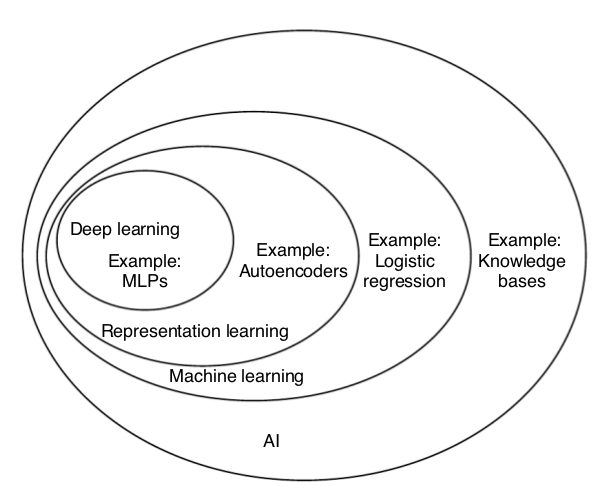
\includegraphics[width=0.7\textwidth]{imgs/AI_venn_diagram.png}
    \caption{Un diagramma di ven che illustra le relazioni tra i diversi sottogruppi dell'intelligenza artificiale, vediamo infatti come
    il deep learning sia un sottogruppo del representation learning, che a sua volta è un sottogruppo del machine learning.\\
    credits: Yoshua Bengio, Ian J. Goodfellow, Aaron Courville 2015, From the book "Deep Learning"\\}
    \label{fig:ai_venn_diagram}
\end{figure}

\subsection{Confronto con le reti neurali biologiche}

Queste strutture matematiche fecero la prima comparsa in un articolo del 1957, pubblicato da Warren McCulloch e Walter Pitts
"A logical calculus of the ideas immanent in nervous activity", articolo che gettò le basi per la costruzione di reti neurali artificiali
come le conosciamo oggi partendo proprio dal sistema nervoso.
Infatti le reti neurali artificiali sono ispirate alle reti neurali biologiche, le quali hanno un comportamento più complesso della
controparte artificiale, la quale deve fare i conti con la complessità computazionale che deve essere ridotta per garantire una elaborazione
efficiente nei calcolatori.
Il neurone biologico componente principale del cervello e del sistema nervoso, è costituito da un corpo cellulare o soma, dai dendriti, 
dall'assone e dalle sinapsi.
    \begin{figure}[H]
        \centering
        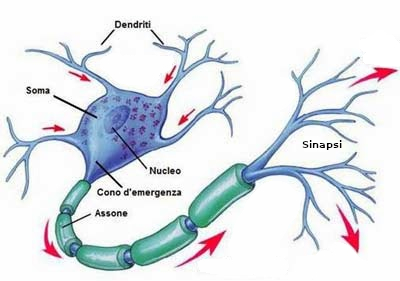
\includegraphics[width=0.5\textwidth]{imgs/neurone.jpg}
        \caption{Schema di un neurone biologico.}
        \label{fig:neuron_bio}
    \end{figure}
Il neurone riceve degli impulsi da altri neuroni o da altri apparati sensoriali attraverso i dendriti, che sono delle strutture ramificate
che si estendono dalla cellula, questi impulsi vengono accumulati all'interno del soma, e se la somma supera un certo valore di soglia
si innesca la propagazione di un'impulso, che viene trasmesso attraverso l'assone verso altri neuroni o verso altri organi.
L'assone è una struttura che si estende dalla cellula, a seconda della tipologia di neurone può estendersi da pochi micrometri fino anche ad un metro,
e presenta all'estremità opposta del soma le sinapsi, le quali consentono la propagazione dell'impulso dall'assone ad altri neuroni.
La struttura dell'assone è rivestita dalla guaina mielinica che ne facilita la conduzione degli impulsi, maggiore è lo spessore della guaina
minore è la resistenza al passaggio dell'impulso, e dunque maggiore sarà l'ampiezza del segnale in uscita a parità di quello di ingresso. 
Tale meccanismo è utilizzato per accumulare informazione nella struttura della rete neurale biologica.

\subsection{Feedforward neural networks}

Uno dei primi modelli ad essere proposti e utilizzati nella pratica è stato quello delle reti neurali feedforward (o multi layer perceptron MLP),
in cui i neuroni sono disposti in strati, e l'output di ogni neurone di uno strato è connesso con l'input di tutti i neuroni dello strato successivo, 
attraverso delle connessioni che conservano un peso, la configurazione di tali pesi determina il comportamento della rete.
Tali reti come dice il nome propagano l'informazione dallo strato di input a quello di output attraverso i layer intermedi,
in modo lineare, senza retropropagazioni intermedie dell'informazione.

    \begin{figure}[H]
        \centering
        \includesvg[width=0.6\textwidth]{imgs/es_nn_1.svg}
        \caption{Esempio di rete neurale feedforward. In tale rete è possibile vedere i neuroni rappresentati dai nodi del grafo, e
        le interconnessioni tra di essi che definiscono il peso o l'importanza di tale connessione.\\
        File:Rete-Neurale2.svg. In Wikipedia. https://commons.wikimedia.org/wiki/File:Rete-Neurale2.svg}
        \label{fig:feedforward_nn}
    \end{figure}

\subsubsection{Il neurone artificiale}

    \begin{wrapfigure}{r}{0.6\textwidth}
        \centering
        \vspace{-25pt}
        \includesvg[width=0.5\textwidth]{imgs/neurone_artificiale.svg}
        \caption{Esempio di Neurone artificiale.}
        \label{fig:artificial_neuron}
        \vspace{0pt}
    \end{wrapfigure}

Il neurone artificiale emula il comportamento del neurone biologico, semplificandone notevolmente la complessità,
una delle più importanti semplificazioni è che il neurone artificiale opera in un regime temporale discreto e non continuo come la controparte.
Il neurone artificiale inoltre non utilizza un meccanismo di accumulazione e spike, ma restituisce un output per ogni input ricevuto,
ciò che varia è l'intensità di questo output, che dipende dall'intensità degli input ricevuti, e dai pesi delle connessioni con tali input.
Il neurone artificiale inoltre è provvisto di una funzione di trasferimento che mappa la somma pesata degli input ricevuti con l'uscita.
Vediamo dunque l'espressione che caratterizza il comportamento di un neurone artificiale:
\begin{equation}
    \label{eq:neuron}
    y = f(P) = f(\vec{\mathbf{w}} \cdot \vec{\mathbf{x}} + b) = f(\sum_{i=1}^{n} w_i x_i + b)
\end{equation}

Considerando $y$ l'output del neurone, $\vec{\mathbf{w}}$ il vettore dei pesi delle connessioni in ingresso, 
$\vec{\mathbf{x}}$ il vettore degli input, $b$ il bias ovvero un valore aggiunto alla somma pesata degli input 
dipendente dal neurone e $f$ la funzione di trasferimento.
La funzione di attivazione o funzione di trasferimento del neurone è la componente che conferisce alla rete la capacità di generare degli output
che hanno una relazione non lineare rispetto agli input ricevuti, e dunque che gli permette di apprendere funzioni non lineari.
La funzione di attivazione solitamente deve essere derivabile, o almeno derivabile a tratti per poter essere utilizzata in un contesto di apprendimento,
in quanto la derivata della funzione di attivazione viene utilizzata per calcolare il gradiente della funzione di errore dall'algoritmo Backpropagation,
e in seguito per aggiornare i pesi da parte della funzione di ottimizzazione (es. SGD).
Di seguito sono mostrate alcune delle più comuni funzioni di attivazione:

    \begin{figure}[H]
        \begin{tabular}{cc}
            % first row
            \vspace{0.15cm}
            \subfloat[Sigmoide]{
                \label{fig:sigmoid}
                \centering
                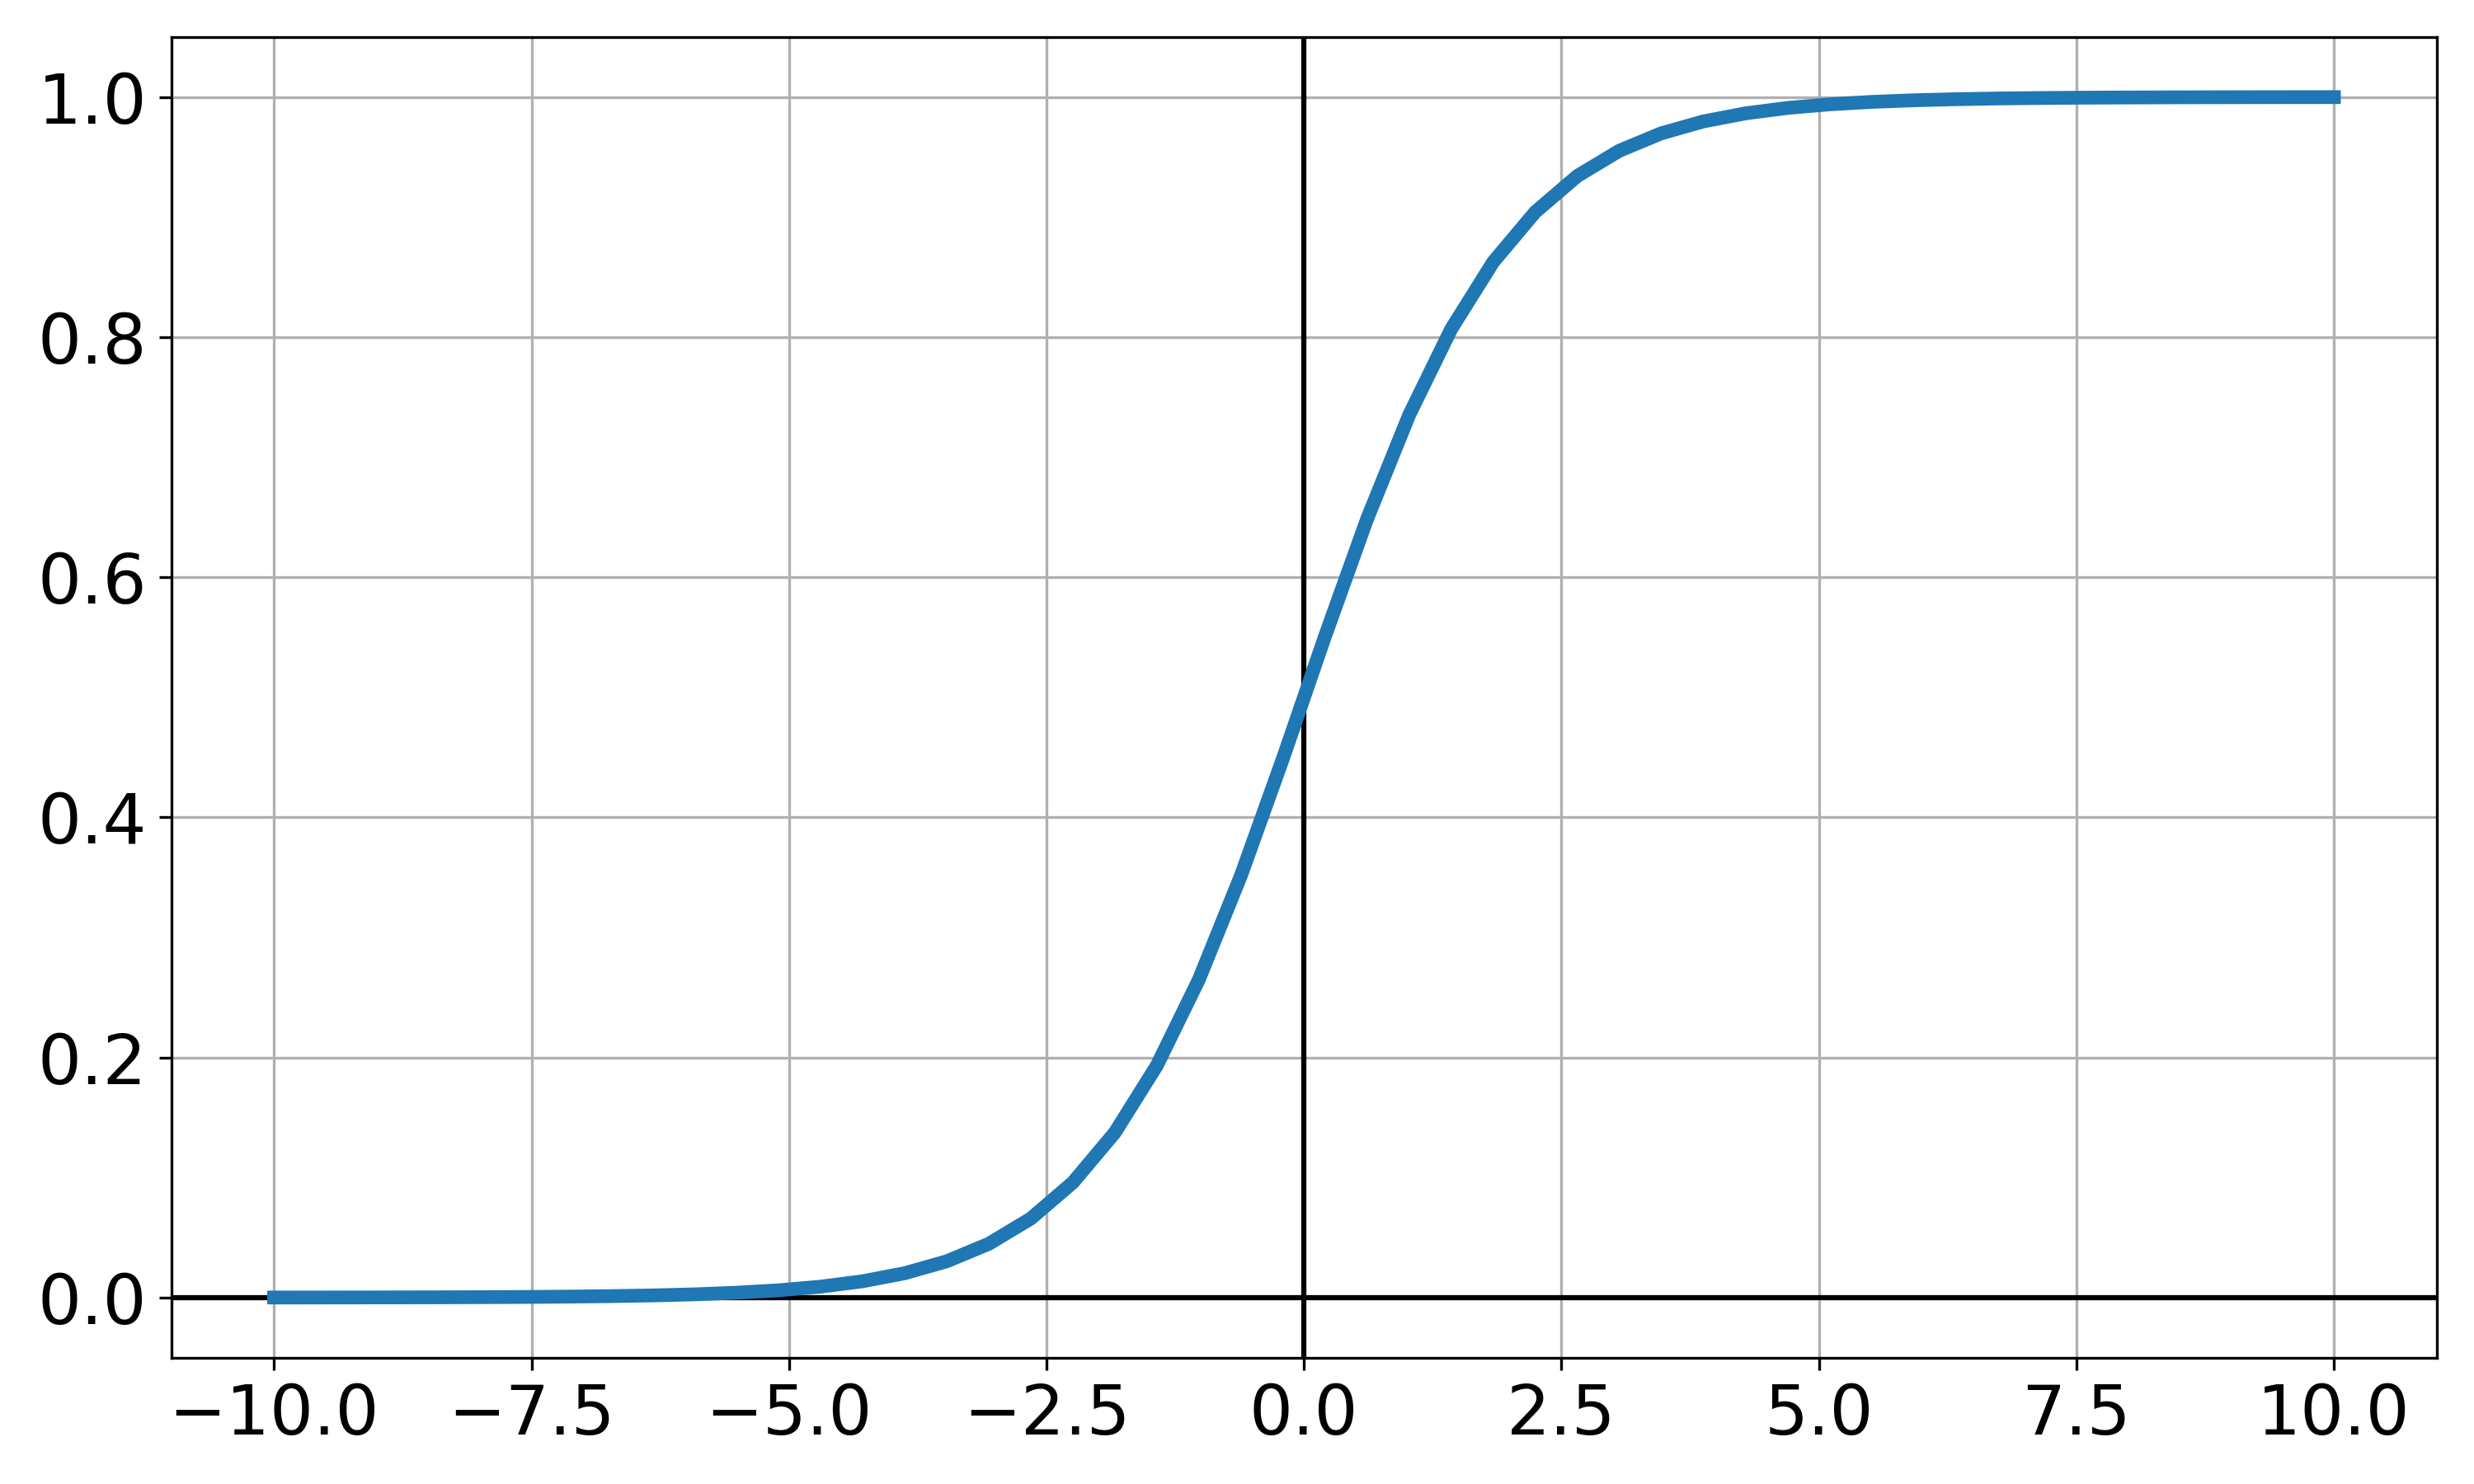
\includegraphics[width=0.4\textwidth]{imgs/activations/sigmoid.png}
            }  &
            \subfloat[Tangente iperbolica]{
                \label{fig:tanh}
                \centering
                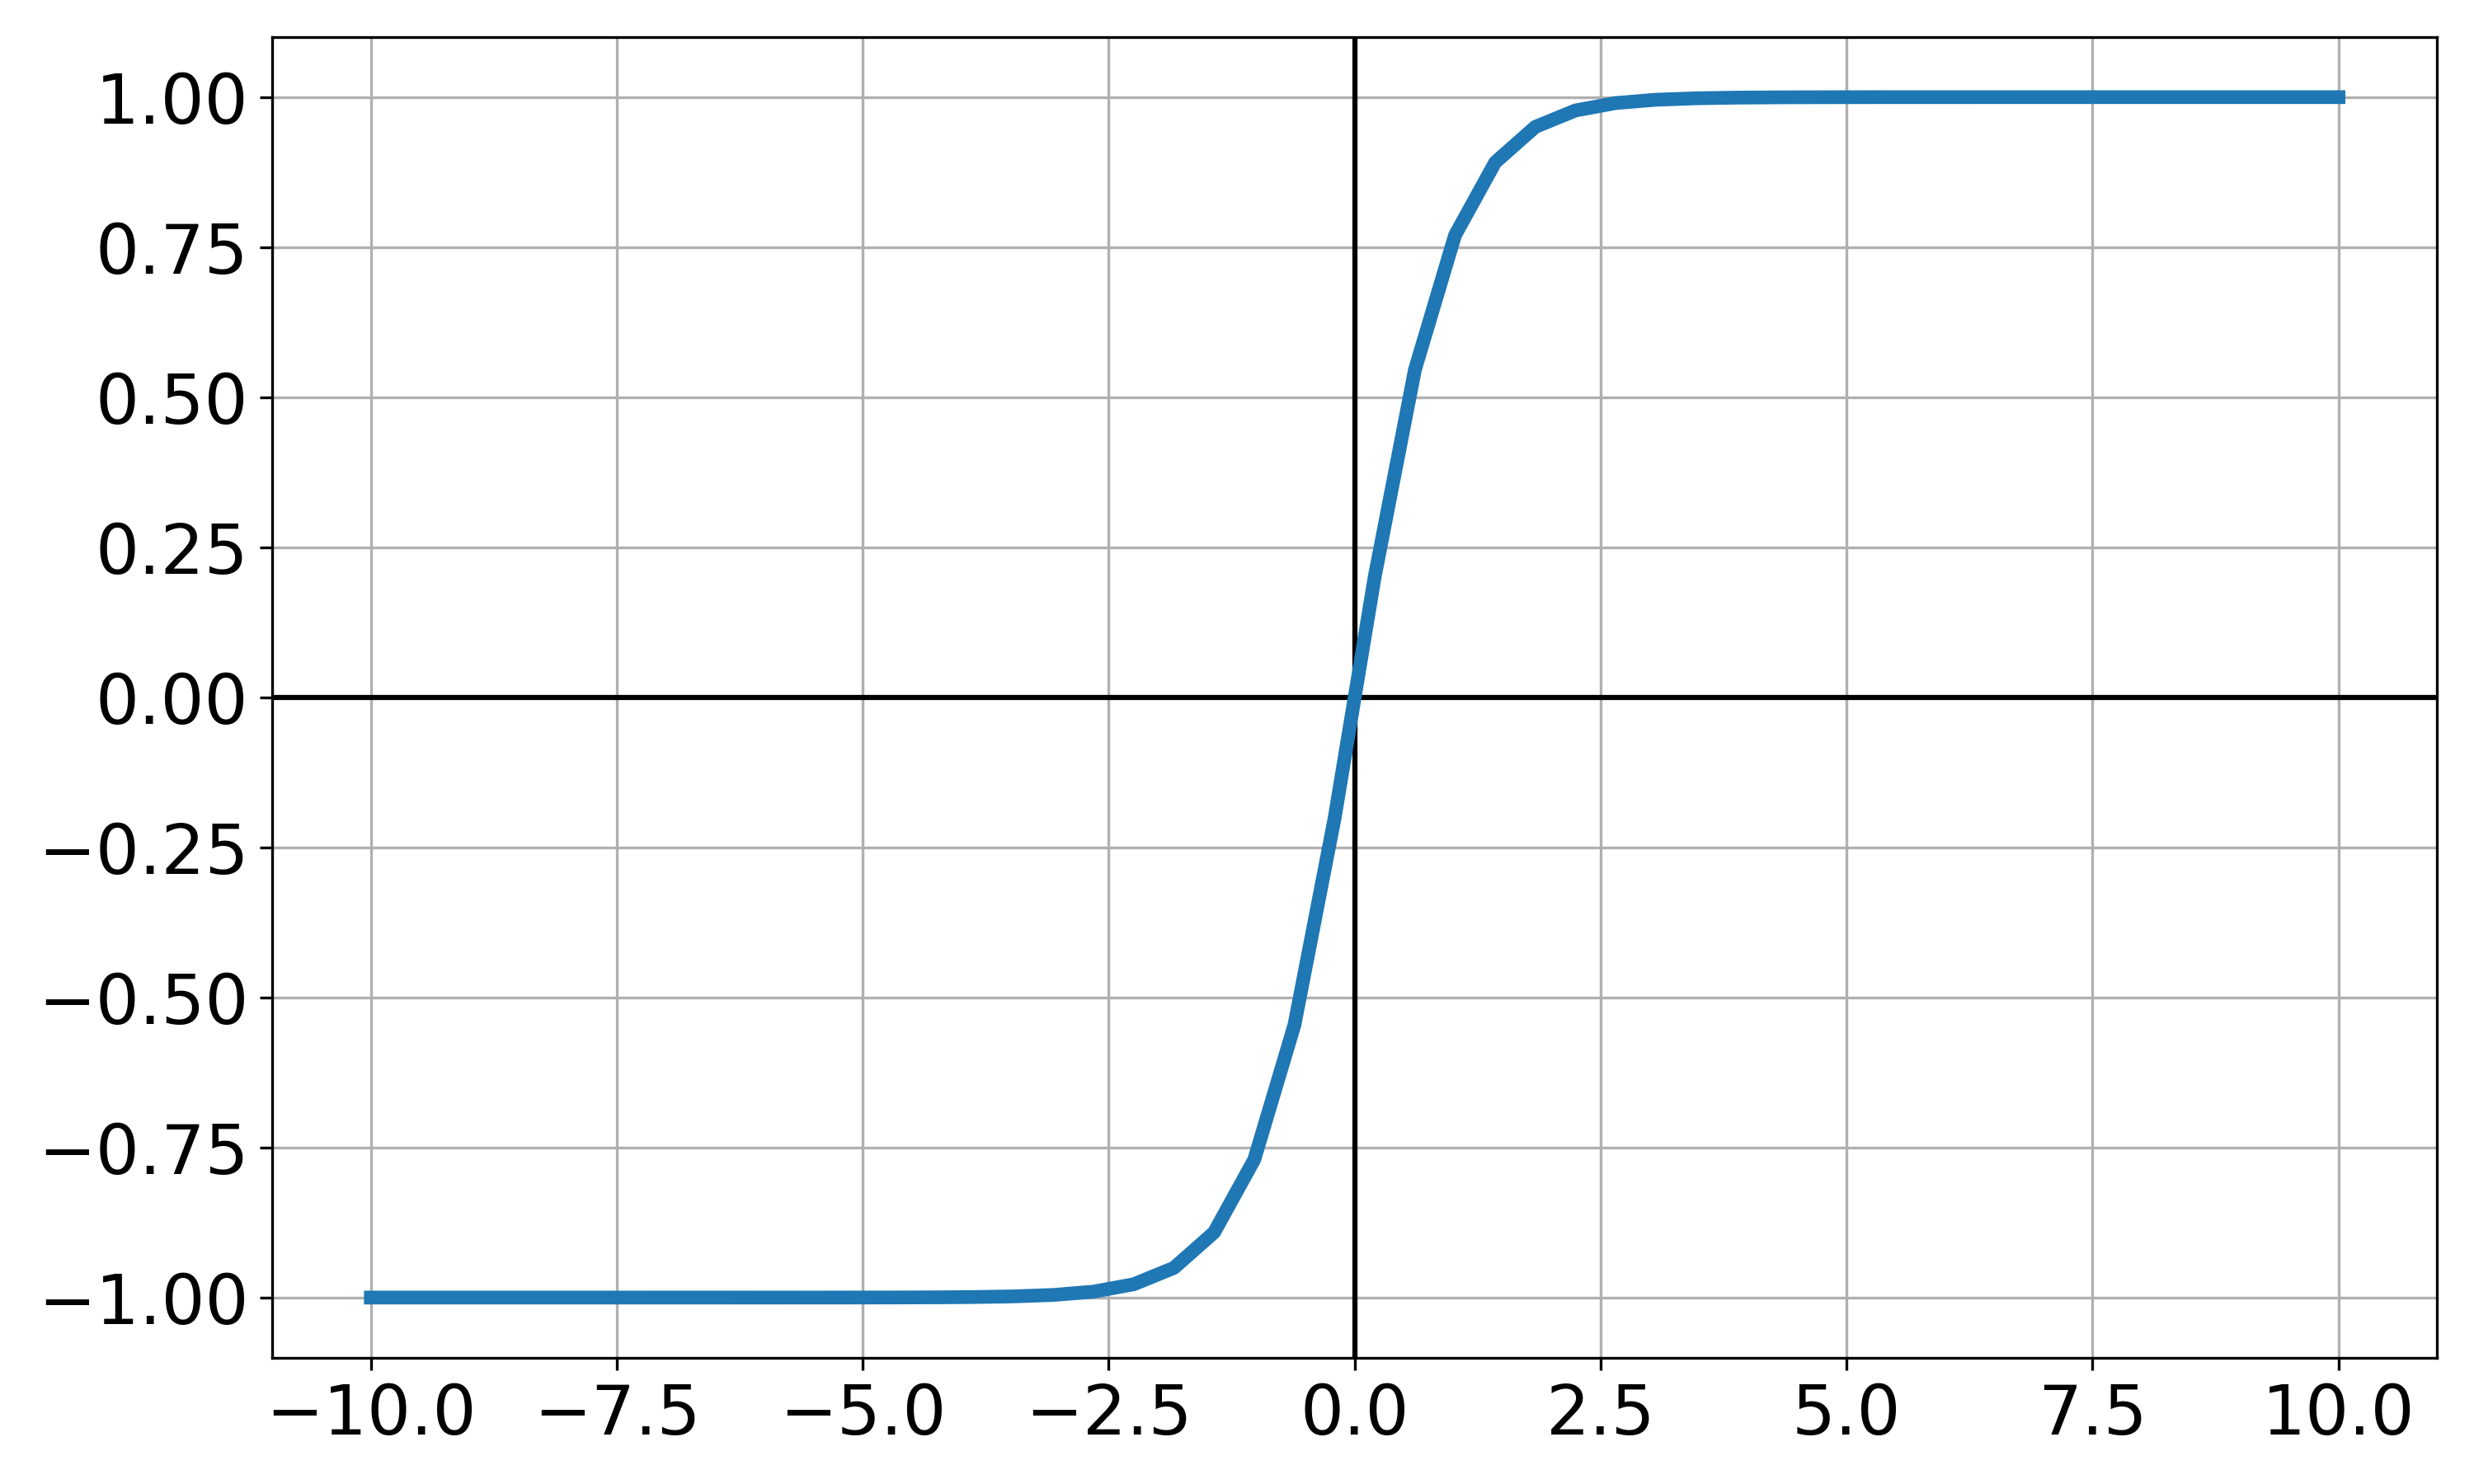
\includegraphics[width=0.4\textwidth]{imgs/activations/tanh.png}
            }  \\
            \vspace{0.25cm}
            \subfloat{
                \begin{tabular}{|c|}
                    \hline
                    $\mathbf{f(x) = \frac{1}{1 + e^{-x}}}$ \\
                    \hline
                \end{tabular}
            } &
            \subfloat{
                \begin{tabular}{|c|}
                    \hline
                    $\mathbf{f(x) = \frac{e^x - e^{-x}}{e^x + e^{-x}}}$ \\
                    \hline
                \end{tabular}
            } \\

            % second row
            \vspace{0.15cm}
            \subfloat[Rectified linear unit (RELU)]{
                \label{fig:relu}
                \centering
                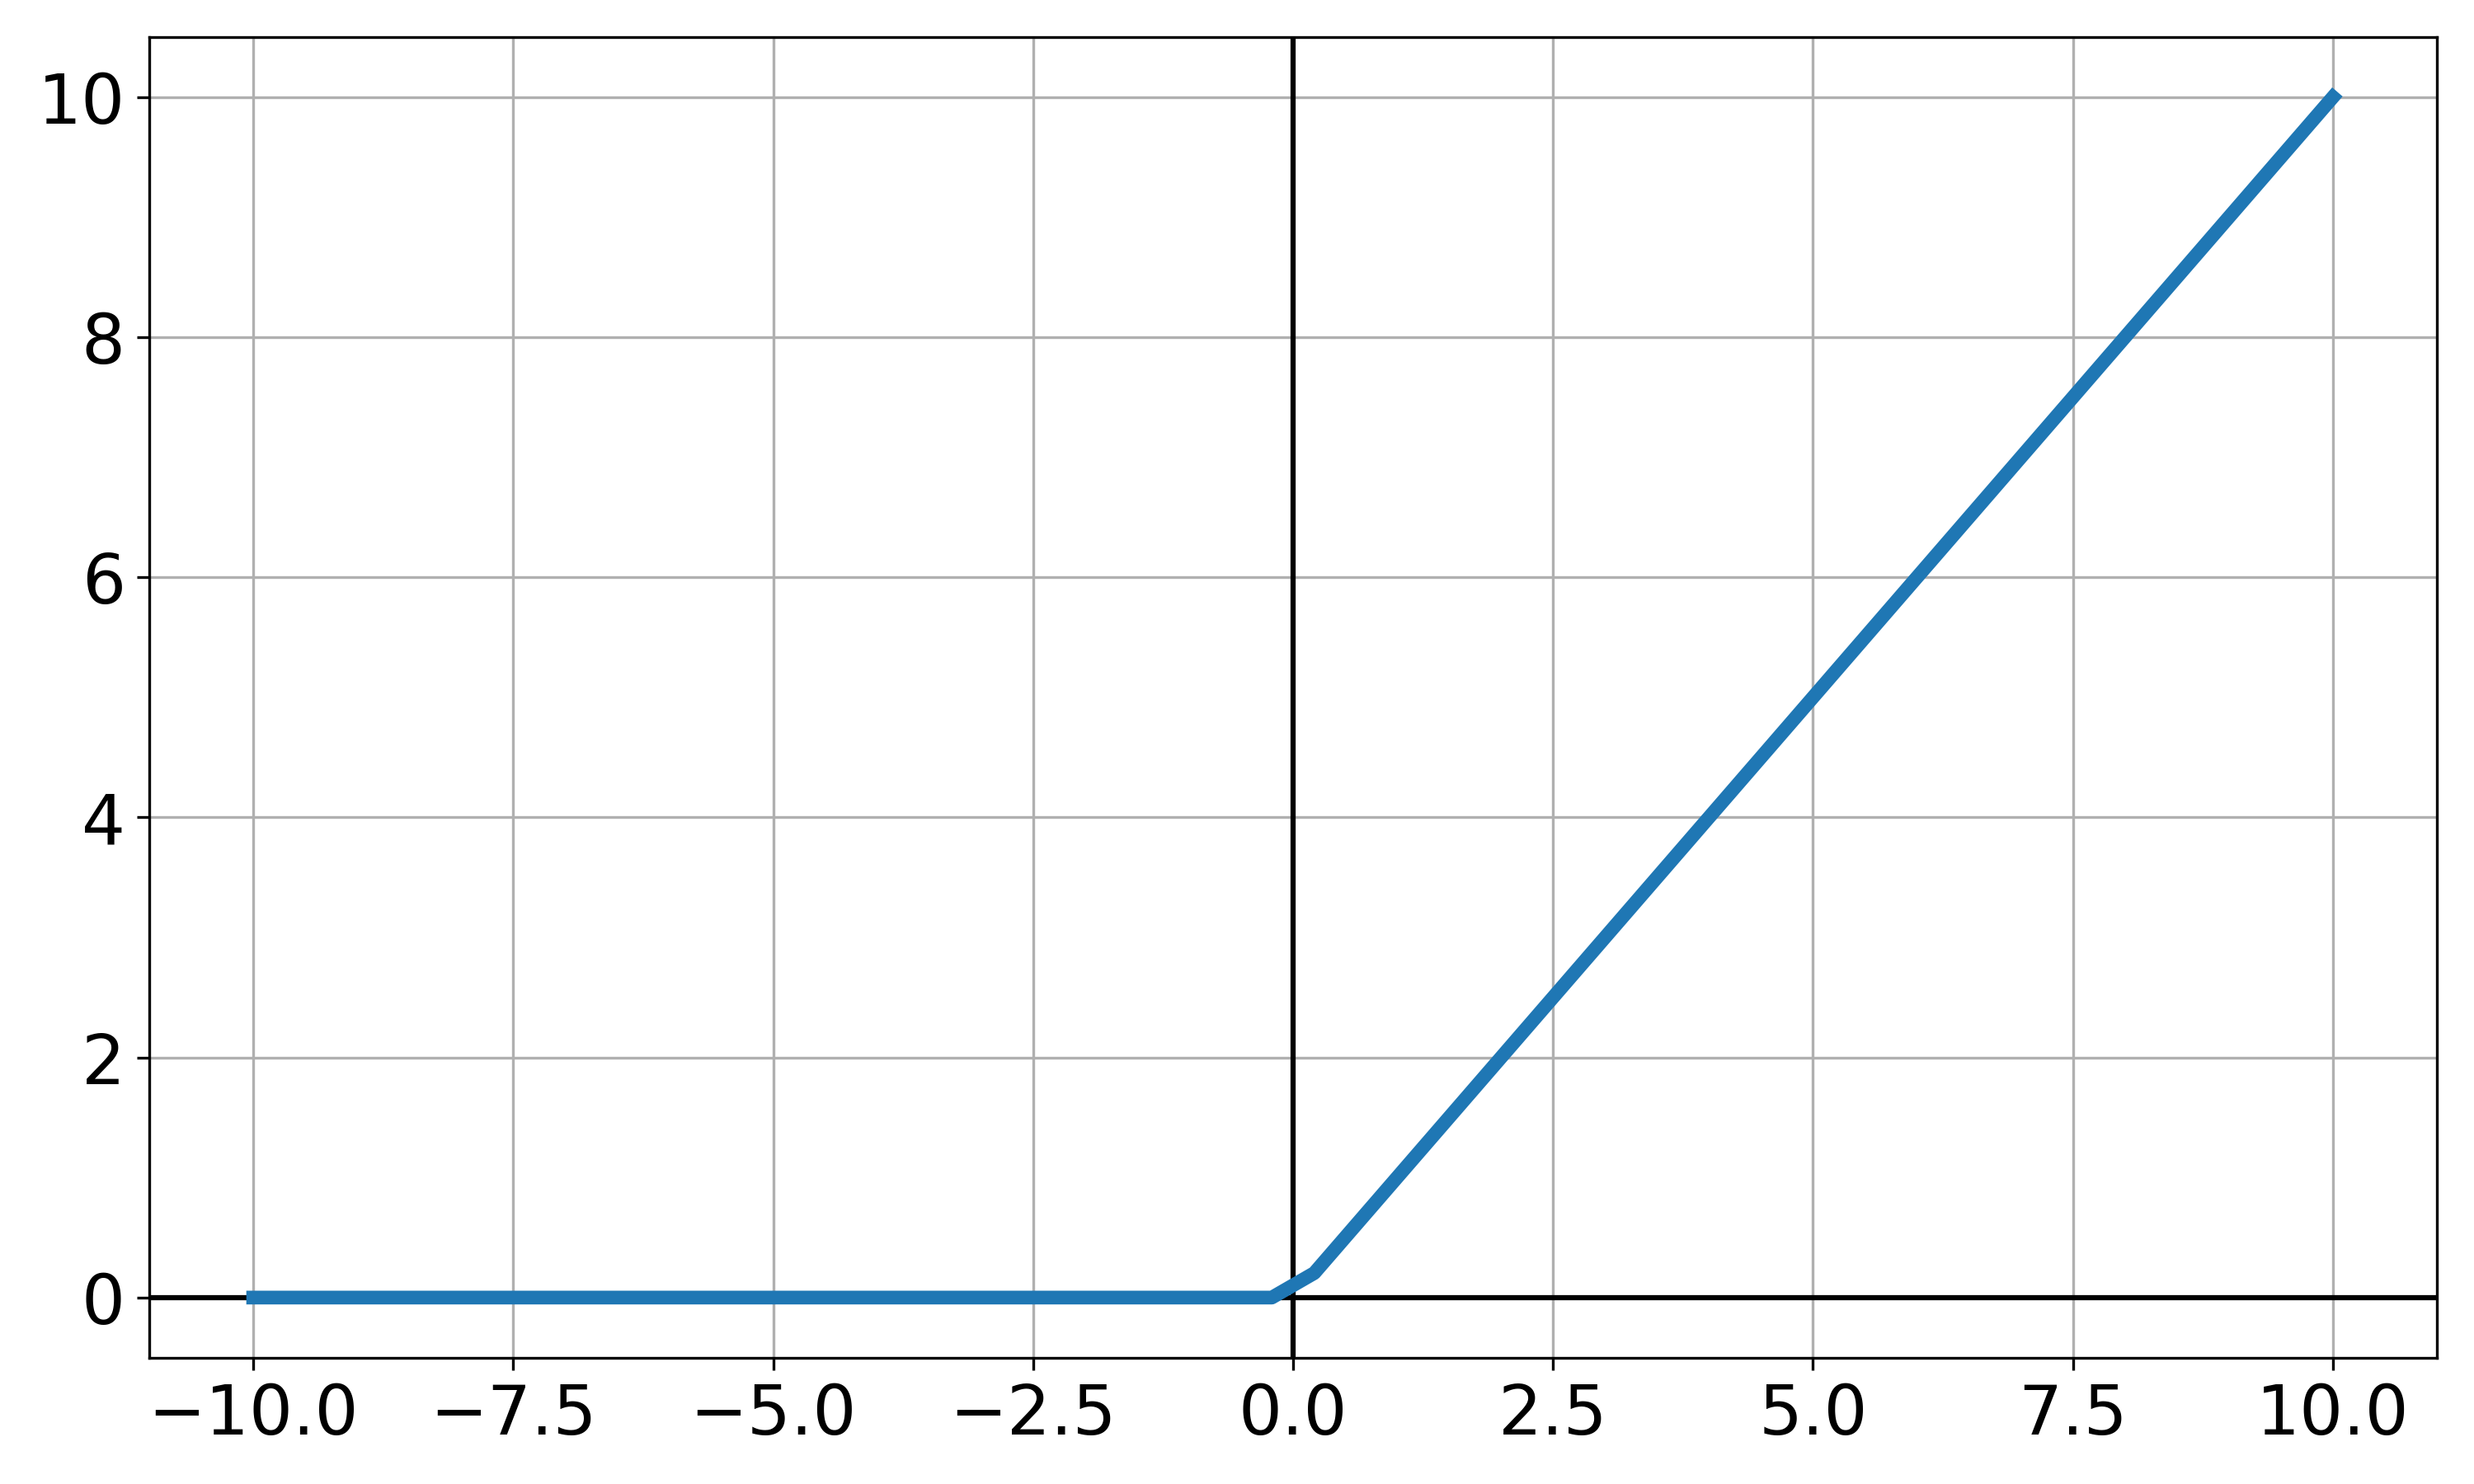
\includegraphics[width=0.4\textwidth]{imgs/activations/relu.png}
            }  &
            \subfloat[Leaky RELU]{
                \label{fig:leaky_relu}
                \centering
                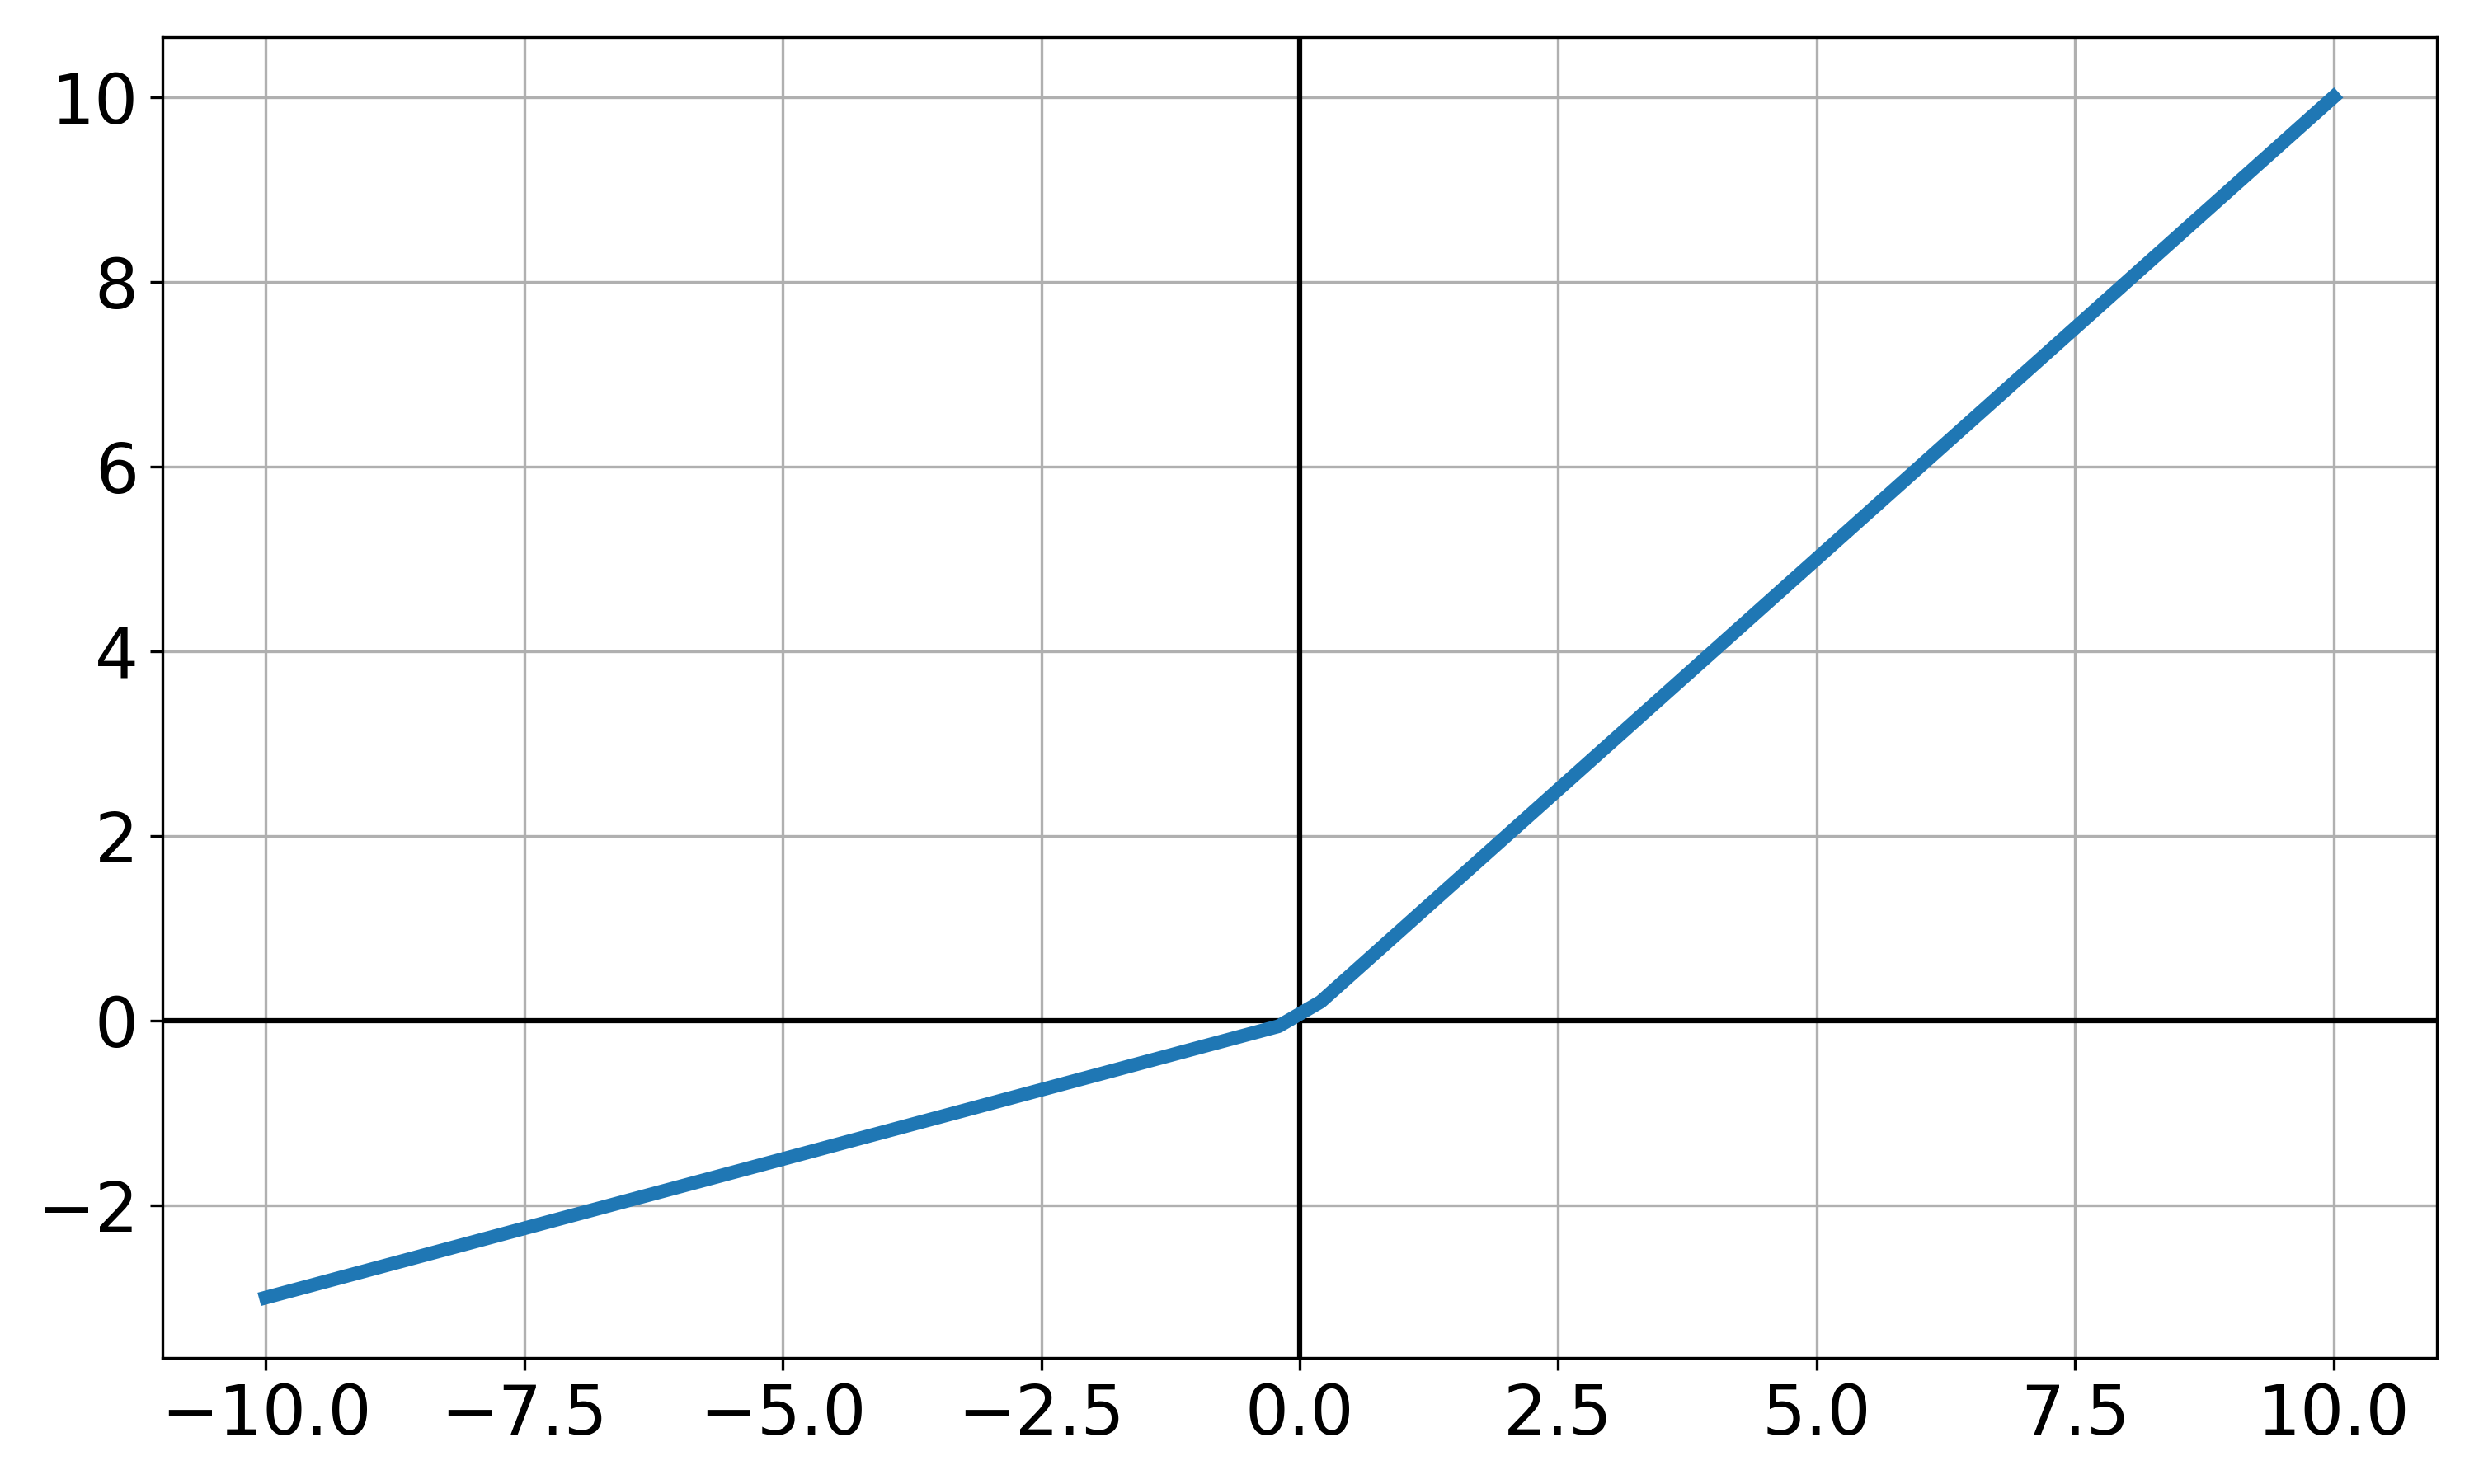
\includegraphics[width=0.4\textwidth]{imgs/activations/leaky_relu.png}
            }  \\
            \vspace{0.25cm}
            \subfloat{
                \begin{tabular}{|c|}
                    \hline
                    $\mathbf{f(x) = \begin{cases} 0 & x < 0 \\ x & x \geq 0 \end{cases}}$ \\
                    \hline
                \end{tabular}
            } &
            \subfloat{
                \begin{tabular}{|c|}
                    \hline
                    $\mathbf{f(x) = \begin{cases} \alpha x & x < 0 \\ x & x \geq 0 \end{cases}}$ \\
                    \hline
                \end{tabular}
            } \\

            % third row
            \vspace{0.15cm}
            \subfloat[Exponential linear unit (ELU)]{
                \label{fig:elu}
                \centering
                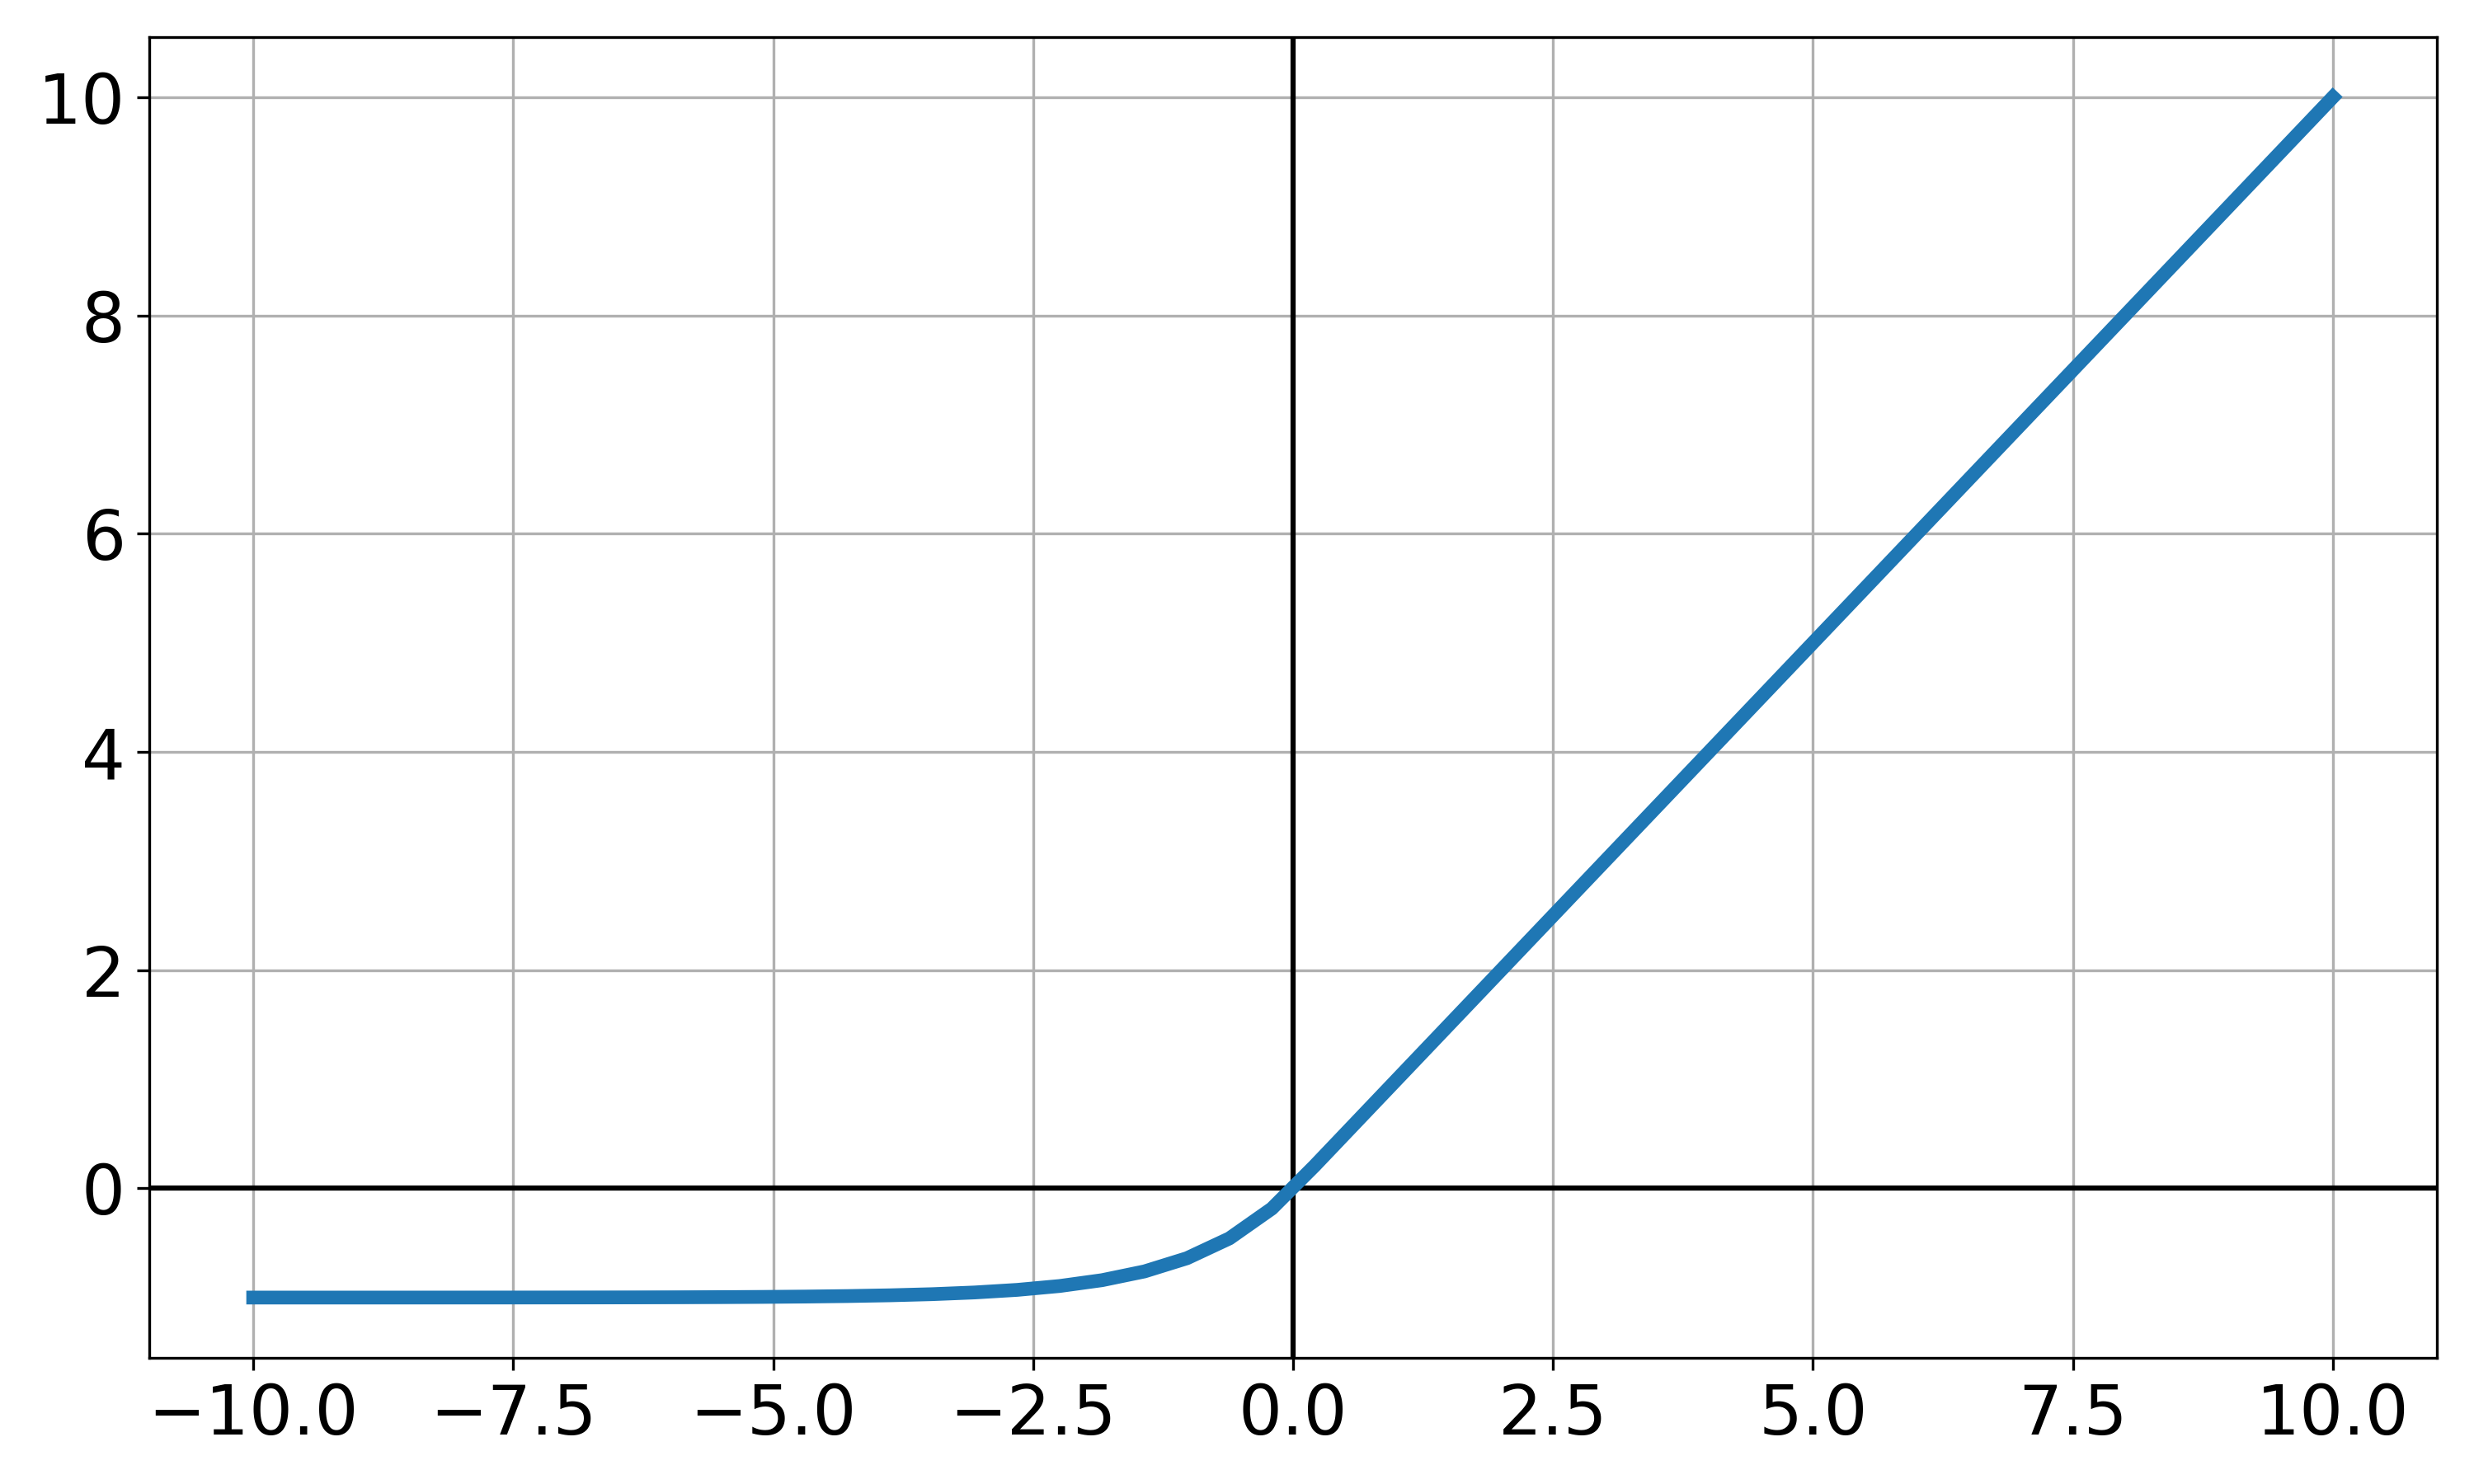
\includegraphics[width=0.4\textwidth]{imgs/activations/elu.png}
            }  &
            \subfloat[Gaussian error linear unit (GELU)]{
                \label{fig:gelu}
                \centering
                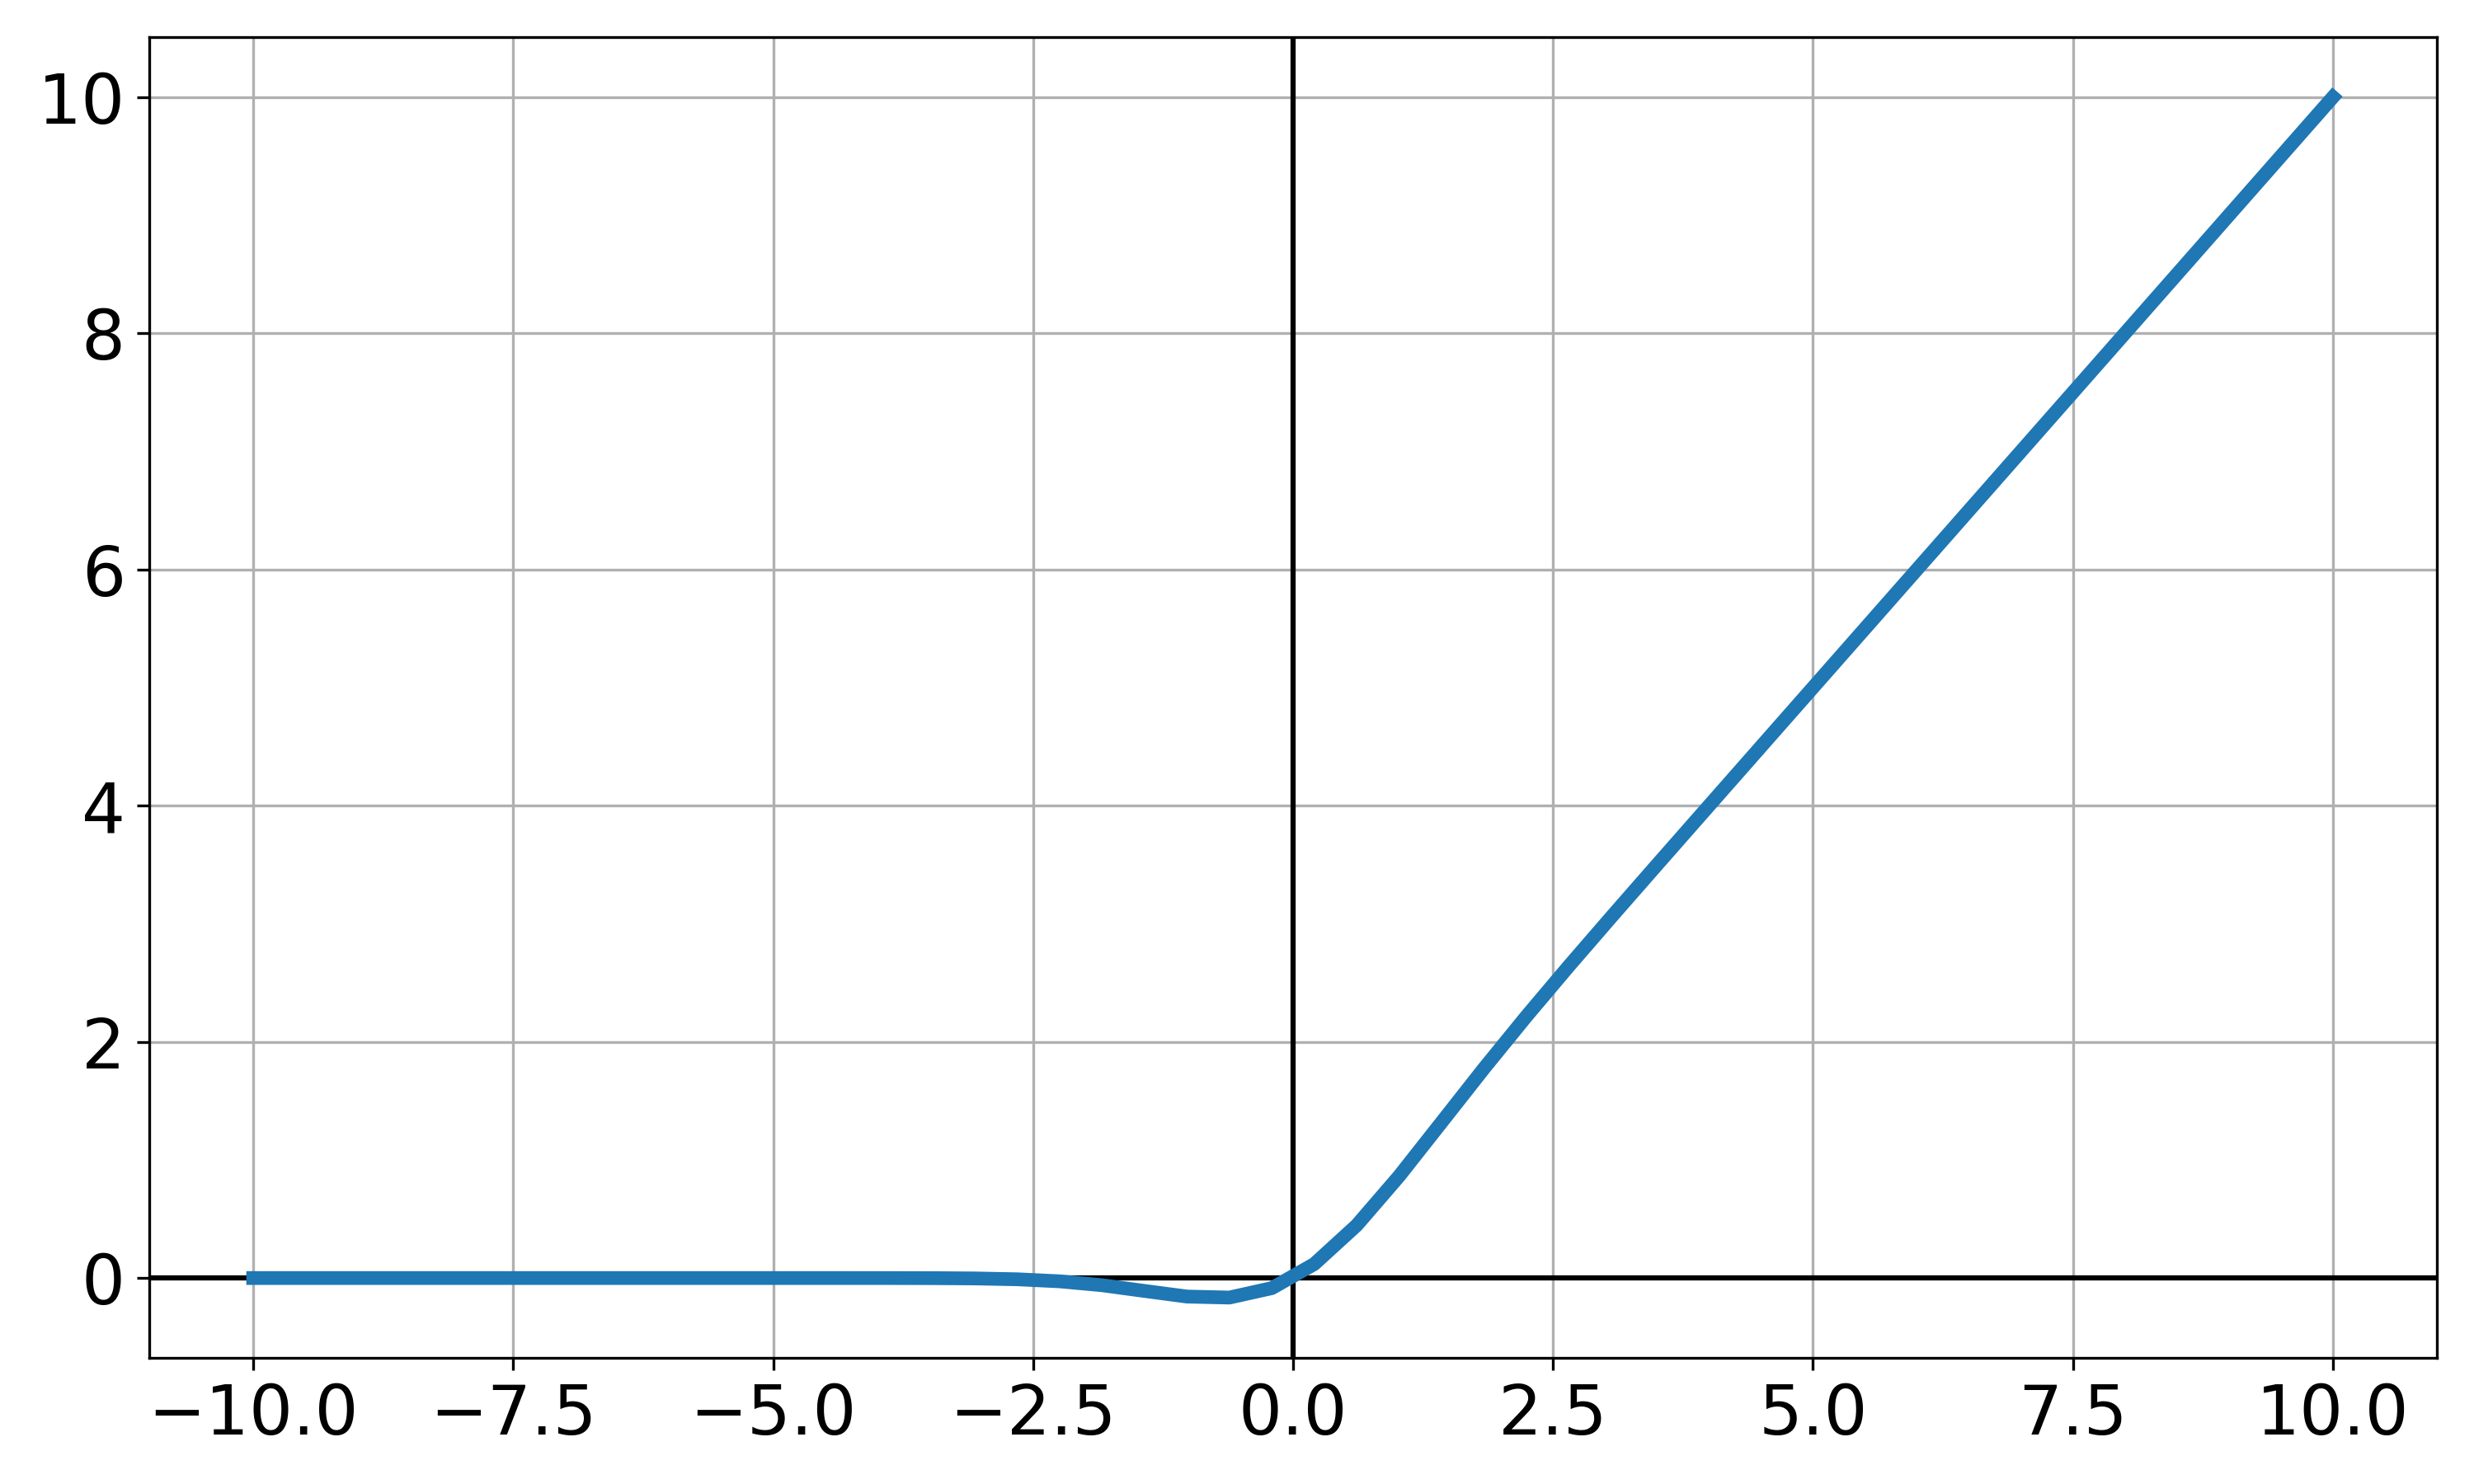
\includegraphics[width=0.4\textwidth]{imgs/activations/gelu.png}
            }  \\
            \vspace{0cm}
            \subfloat{
                \begin{tabular}{|c|}
                    \hline
                    $\mathbf{f(x) = \begin{cases} x & \text{if } x \geq 0 \\ \alpha(e^x - 1) & \text{if } x < 0 \end{cases}}$ \\
                    \hline
                \end{tabular}
            } &
            \subfloat{
                \begin{tabular}{|c|}
                    \hline
                    $\mathbf{f(x) = x*\Phi(x)}$ \\
                    \hline
                \end{tabular}
            } \\
        \end{tabular}
    \end{figure}
La sigmoide e la tangente iperbolica, sono funzioni molto vecchie utilizzate
sin dai primi anni '90, ma sono state sostituite da funzioni più moderne e semplici da calcolare, come le funzioni RELU e Leaky RELU.
Vengono ancora utilizzate però in casi particolari come nello stadio finale di una rete neurale, quando si ha bisogno di un output che sia compreso tra 0 e 1.
Le funzioni ELU e GELU sono invece funzioni di attivazione più recenti, che vengono utilizzate per migliorare l'apprendimento delle reti neurali
in casi specifici, ma in generale RELU e Leaky RELU sono le funzioni più utilizzate, in quanto offrono un buon compromesso tra prestazioni e accuratezza.

\subsubsection{Il Back-propagation}

La prima volta che questo algoritmo fu proposto fu nel 1986 da David E. Rumelhart, Geoffry E. Hinton e Ronald J. Williams, su nature
con l'articolo \textit{Learning representations by back-propagating errors}.
Questo algoritmo ha segnato da quel momento una vera e propria rivoluzione nel campo dell'apprendimento automatico, rendendo possibile l'addestramento dei
modelli neurali come li conosciamo oggi e plasmando lo scenario attuale dell'intelligenza artificiale.

Ciò che questo algoritmo fa effettivamente è calcolare il gradiente della funzione di errore nello spazio dei pesi di una rete neurale, 
partendo dal layer di uscita e andando a calcolare il gradiente per ogni layer precedente fino ad arrivare al layer di input, tale gradiente può essere poi
utilizzato per aggiornare i pesi della rete attraverso una funzione di ottimizzazione, in modo da minimizzare o massimizzare la funzione di costo che si vuole ottimizzare.

Da un punto di vista matematico, data la precedente definizione di neurone e rete neurale, possiamo definire una rete neurale come una funzione $\mathbf{g(x)}$
come combinazione di composizione di funzioni e moltiplicazioni di matrici.

\begin{equation}
    \mathbf{\vec{y} = g(\vec{x}) = f_{L}(\mathbf{W^{L} \cdot f^{L-1}(W^{L-1} \cdot f^{L-2}(\dots W^{3} \cdot f^{2}(W^{2} \cdot f^{1}(W^{1} \cdot \vec{x})) \dots ))})}
\end{equation}

Dove $\mathbf{f_{L}}$ è la funzione di attivazione del layer di uscita, $\mathbf{f_{i}}$ è la funzione di attivazione del layer $i$ e $\mathbf{W^{i}}$ è la matrice dei pesi del layer $i$.
Abbiamo inoltre che $\mathbf{\vec{x}}$ e $\mathbf{\vec{y}}$ sono rispettivamente il vettore di input e il vettore di output della rete neurale, se consideriamo
$\mathbf{\hat{y}}$ il vettore di output desiderato, possiamo definire la funzione di costo. In questo caso utilizzeremo la loss MSE (Mean Squared Error), ma
si può sostituire con qualsiasi funzione di costo.

\begin{equation}
    \mathbf{E = \frac{1}{n} \sum_{i=1}^{n} (\hat{y_{i}} - y_{i})^2}
\end{equation}

A questo punto data una determinata coppia di input e output ($\mathbf{\vec{x}}$, $\mathbf{\vec{y}}$), possiamo calcolare il gradiente della funzione di costo
attraverso la \textit{regola della catena}, che ci permette di calcolare il gradiente della funzione di costo per ogni peso della rete.

\begin{equation}
    \mathbf{\frac{\partial E}{\partial w^{l}_{ij}} = \frac{\partial E}{\partial a^{l}} \cdot \frac{\partial a^{l}}{\partial z^{l}} \cdot \frac{\partial z^{l}}{\partial w^{l}_{ij}}}
\end{equation}

Otteniamo così il gradiente della funzione di costo per il peso $w^{l}_{ij}$ appartenente al layer $l$, al neurone $i$ e alla sinapsi $j$.

Per l'esecuzione dell'algoritmo back propagation è necessario effettuare il caching dei valori intermedi calcolati durante il passaggio in avanti,
nello specifico degli input pesati dei neuroni prima della funzione di attivazione $\mathbf{\vec{z}^{l}}$ e l'output dei neuroni dopo la funzione di attivazione $\mathbf{\vec{a}^{l}}$
per ogni layer.

Consideriamo la derivata della funzione di errore rispetto all'input del modello:

\begin{equation}
    \mathbf{\frac{\partial E}{\partial x} = (\frac{\partial E}{\partial a^{L}}) \circ (\frac{\partial a^{L}}{\partial z^{L}} \cdot \frac{\partial z^{L}}{\partial a^{L-1}}) \circ (\frac{\partial a^{L-1}}{\partial z^{L-1}} \cdot \frac{\partial z^{L-1}}{\partial a^{L-2}}) \circ \dots \circ (\frac{\partial a^{2}}{\partial z^{2}} \cdot \frac{\partial z^{2}}{\partial a^{1}}) \circ (\frac{\partial a^{1}}{\partial z^{1}} \cdot \frac{\partial z^{1}}{\partial x})}
\end{equation}

Dove $\mathbf{\circ}$ è il prodotto di Hadamard, un semplice prodotto element-wise tra matrici di dimensioni uguali, che moltiplica elemento per elemento le due matrici.
Osservando questa formulazione della derivata possiamo notare che $\mathbf{\frac{\partial a^{L}}{\partial z^{L}} \cdot \frac{\partial z^{L}}{\partial a^{L-1}}}$ è la derivata della funzione di attivazione 
moltiplicata per la matrice dei pesi del layer stesso. 
Inoltre possiamo riscrivere la derivata $\mathbf{\frac{\partial E}{\partial a^{L}}}$ in termini di gradiente
$\mathbf{\nabla_{a} E}$, invertendo l'ordine dei prodotti e trasponendo le matrici:

\begin{equation}
    \mathbf{\nabla_{x} E = (W^1)^T \cdot (f^1)' \circ \dots \circ (W^{L-1})^T \cdot (f^{L-1})' \circ (W^{L})^T \cdot (f^{L})' \circ \nabla_{a^L} E}
\end{equation}

A questo punto possiamo introdurre i prodotti parziali del gradiente per determinare il gradiente della funzione di errore ad un determinato layer $l$:

\begin{equation}
    \mathbf{\delta^{l} = (f^{l})' \circ (W^{l+1})^T \cdot (f^{l+1})' \circ \dots \circ (W^{L})^T \cdot (f^{L})' \circ \nabla_{a^L} E}
\end{equation}

E notiamo che ogni prodotto parziale può essere definito come il prodotto tra il gradiente e la matrice trasposta dei pesi del layer successivo per
la derivata della funzione di attivazione del layer stesso.

\begin{equation}
    \mathbf{\delta^{l-1} = (f^{l-1})' \circ (W^{l})^T \cdot \delta^{l}}
\end{equation}

Quindi:

    $\mathbf{\delta^{L} = (f^{L})' \circ \nabla_{a^L} E}$

    $\mathbf{\delta^{L-1} = (f^{L-1})' \circ (W^{L})^T \cdot \delta^{L} = (f^{L-1})' \circ (W^{L})^T \cdot (f^{L})' \circ \nabla_{a^L} E}$

    $\dots$

    $\mathbf{\delta^{2} = (f^{2})' \circ (W^{3})^T \cdot \delta^{3} = (f^{2})' \circ (W^{3})^T \cdot \dots \circ (W^{L})^T \cdot (f^{L})' \circ \nabla_{a^L} E}$

    $\mathbf{\delta^{1} = (f^{1})' \circ (W^{2})^T \cdot \delta^{2} = (f^{1})' \circ (W^{2})^T \cdot (f^{2})' \circ (W^{3})^T \cdot \dots \circ (W^{L})^T \cdot (f^{L})' \circ \nabla_{a^L} E}$

In tal modo possiamo calcolare i prodotti parziali del gradiente per ogni layer, partendo dallo strato di output all'indietro, minimizzando così il numero di operazioni
richieste per il calcolo del gradiente. Per ottenere i gradienti dei pesi è sufficiente moltiplicare il prodotto parziale del gradiente per l'output del layer precedente:

\begin{equation}
    \mathbf{\nabla_{w^{l}} E = \delta^{l} \cdot (a^{l-1})^T}
\end{equation}

L'oggetto $\mathbf{\nabla_{w^{l}} E}$ rappresenta una matrice della stessa dimensione della matrice dei pesi del layer $l$, contenente i gradienti della funzione di errore di tali pesi,
mentre $a^{l-1}$ è l'output di tutte le unità del layer precedente.

\begin{wrapfigure}{r}{0.5\textwidth}
    \centering
    \hspace{-25pt}
    %\vspace{-25pt}
    \includesvg[width=0.4\textwidth]{imgs/backpropagation.svg}
    \caption{Esempio di retropropagazione su di una rete semplificata a 2 strati.}
    \label{fig:backpropagation}
    \vspace{35pt}
\end{wrapfigure}

Si consideri che è possibile scomporre un elemento della matrice $\mathbf{\nabla_{w^{l}} E}$ nel seguente modo:
\begin{equation}
    % TODO: VERIFICARE SE QUESTA EQUAZIONE È CORRETTA
    \mathbf{\nabla_{w^{l}} E_{k,k} = \frac{\partial E}{\partial w_{k,k}^{l}}} 
\end{equation}

Tale gradiente a questo punto può essere utilizzato per aggiornare il peso $w_{k,k}^{l}$,
applicando un semplice coefficiente di apprendimento $\eta$:
\begin{equation}
    \mathbf{W_{k,k}^1 = W_{k,k}^1 + \Delta W_{k,k}^1}
\end{equation}
\begin{equation}
    \mathbf{\Delta W_{k,k}^1 = - \eta \cdot \nabla_{w^1}E_{k,k}}
\end{equation}

é importante notare che questo è un'approccio molto basilare, che può essere migliorato attraverso l'uso di tecniche di ottimizzazione
più evolute come ad esempio l'ottimizzazione SGD (Stochastic Gradient Descent) o l'ottimizzazione ADAM.

\subsubsection{Teorema di approssimazione universale}

Le reti neurali artificiali, non hanno dimostrato solo nella pratica con risultati sperimentali la loro efficacia nel risolvere
i problemi, ma anche nella teoria, infatti in molti studi è stata provata la loro efficacia come approssimatori universali.
Quando si parla di approssimatori universali ci si riferisce a delle funzioni che possono approssimare su un dato intervallo di valori
qualunque altra funzione continua. Nel caso particolare delle reti neurali vi è una grande quantità di varianti, per le quali
si ha una diversa dimostrazione per tale proprietà.

Tra i più importanti nel 1989 George Cybenko in \textit{Approximation by superpositions of a sigmoidal function} \cite{cybenko1989approximation},
dimostrò che la sovrapposizione di un numero finito di istanze di una singola funzione univariata può approssimare qualsiasi funzione continua 
di n variabili con supporto nell'ipercubo unitario. Questo risultato permette di asserire che ogni funzione continua può essere approssimata da 
una rete neurale MLP (feedforward) avente uno strato nascosto con un numero finito di unità, con come funzione di attivazione una funzione sigmoide arbitraria.
Di seguito il relativo teorema:
\begin{theorem}
    \label{thm:cybenko_1}
    Sia $sigma$ qualsiasi funzione sigmoide arbitraria. Le sommatorie finite della forma
    \begin{equation}
        \mathbf{G(x) = \sum_{i=1}^{N} \alpha \cdot \sigma(y_i^Tx + \Theta_i)}
    \end{equation}
    sono dense in $C(I_n)$. In altre parole, data qualunque $f \in C(I_n)$ e $\epsilon > 0$ esiste una somma $G(x)$
    con la forma sopra descritta tale che:
    \begin{equation}
        \mathbf{|G(x) - f(x)| < \epsilon \quad \forall x \in I_n}
    \end{equation}
\end{theorem}

Con questo teorema Cybenko dimostra che una rete neurale MLP con un solo strato nascosto può approssimare qualsiasi funzione continua
ma non è in grado di stabilire quante unità deve avere,  in base alla complessità della funzione da approssimare il numero potrebbe essere astronomico.
Altre ricerche negli anni seguenti hanno studiato molteplici varianti di questo teorema, ad esempio per neuroni con funzione di attivazione RELU 
o il caso con profondita del modello arbitraria.

\subsection{Convolutional neural networks}
\begin{comment}
    indice sotto sezione:
    - Storia delle CNN
    - La convoluzione
        - 
    - 

\end{comment}
Le CNN sono reti neurali artificiali molto adatte all'analisi delle immagini, 
la loro struttura è simile a quella che si trovano nel nervo ottico degli organismi viventi.
Sono dette anche \textit{Shift invariant artificial neural networks} (SIANN) in quanto sono 
sono resistenti alla traslazione dell'input per via della loro struttura.

\subsubsection{Storia delle CNN}

La prima pubblicazione alla quale si deve l'invenzione delle CNN è stato un lavoro di David Hunter Hubel e Torsten Wiesel 
\textit{"Receptive fields of single neurones in the cat's striate cortex"}, i quali nel 1959 hanno studiato la struttura della 
corteccia visiva del cervello di un gatto, scoprendo che tali neuroni avevano una struttura particolare, che li rendeva 
soggetti agli stimoli di una certa porzione di retina, detta \textit{campo ricettivo}, tale area era regolare per tutti i neuroni
e tutti avevano una certa sovrapposizione dei rispettivi campi ricettivi.

Il primo lavoro a sfruttare i concetti appresi da Hubel e Wiesel è stato quello di Kunihiko Fukushima il quale nel 1980
ha pubblicato il suo lavoro \textit{Neocognitron}, un sistema di riconoscimento di immagini, utilizzato per la prima volta
per il riconoscimento di numeri scritti a mano in giapponese. 
Sempre a Fukushima si deve anche l'introduzione della funzione di trasferimento \textit{RELU}, precedentemente discussa.

Seguì poi il lavoro di Alex Waibel \textit{"Phoneme Recognition Using Time-Delay Neural Networks"} nel 1987, che segno un'ulteriore passo
nella direzione delle CNN, introducendo per la prima volta l'invarianza alla traslazione. Questo lavoro però
non era focalizzato sulle immagini ma sull'analisi del suono, in particolare il riconoscimento di fonemi.
Ma l'utilizzo di questo modello su 2 dimensioni, ovvero il tempo e la frequenza, lo rendeva concettualmente adatto 
anche all'analisi delle immagini.

In fine il lavoro che ha portato alla nascita delle CNN moderne è stato quello di Yann LeCun
\textit{"Backpropagation applied to handwritten zip code recognition"}, pubblicato nel 1989, in cui è stato utilizzato
il backpropagation per l'addestramento di una rete convoluzionale per il riconoscimento di numeri scritti a mano.

\subsubsection{title}


